\documentclass[11pt,a4paper]{article}
% Replace these fields when initializing a project.
% Keep the short title brief enough to fit in the running header.
\newcommand{\ReportTitle}{Random k-SAT}
\newcommand{\ReportSubtitle}{Satisfiability, algorithms and practical computation}
\newcommand{\ReportAuthor}{Research survey prepared with Codex}
\newcommand{\ReportDate}{11 October 2026\quad |\quad Version 1.1}
\newcommand{\ReportShortTitle}{Random k-SAT}
\newcommand{\ReportSeries}{LITERATURE SURVEY}
\newcommand{\ReportStatus}{Scope and evidence}
\newcommand{\ReportSummary}{%
  When do random Boolean constraints admit a solution? How can one find it,
  or certify that none exists? A survey of threshold theorems, algorithmic
  guarantees, practical solver performance and GPU acceleration, with a
  comparison to phase transitions in convex geometry.}
\newcommand{\ReportScope}{%
  Targeted literature review through 10 October 2026. Published results,
  recent preprint claims and empirical observations are identified separately.
  Reported benchmarks are from the cited authors; no solver benchmark or
  independent mathematical refereeing was performed for this survey.}

% Enable only after adding real BibTeX entries and citations.
\newif\ifreportbibliography
\reportbibliographytrue

\usepackage[T1]{fontenc}
\usepackage[utf8]{inputenc}
\usepackage{amsmath,amsthm,mathtools}
\usepackage{newpxtext,newpxmath}
\usepackage[margin=27mm,headheight=16pt]{geometry}
\usepackage{microtype}
\usepackage{booktabs,tabularx,longtable,array}
\usepackage{enumitem}
\usepackage{graphicx,xcolor}
\usepackage{pgfplots}
\pgfplotsset{compat=1.18}
\usepackage[font=small,labelfont=bf]{caption}
\usepackage[numbers,square,sort&compress]{natbib}
\usepackage{fancyhdr,titlesec,needspace,xurl}

\definecolor{ink}{HTML}{183549}
\definecolor{teal}{HTML}{246A72}
\definecolor{pale}{HTML}{EDF3F5}
\definecolor{muted}{HTML}{53636E}
\usepackage[colorlinks=true,linkcolor=ink,citecolor=ink,urlcolor=teal]{hyperref}
\hypersetup{pdftitle={\ReportTitle},pdfauthor={\ReportAuthor},
  pdfsubject={\ReportSubtitle}}

\titleformat{\section}{\Large\bfseries\color{ink}}{\thesection}{0.7em}{}
\titleformat{\subsection}{\large\bfseries\color{ink}}{\thesubsection}{0.7em}{}
\titlespacing*{\section}{0pt}{2.5ex plus 1ex}{1ex}
\titlespacing*{\subsection}{0pt}{2ex plus .6ex}{.6ex}
\pagestyle{fancy}
\fancyhf{}
\fancyhead[L]{\small\textsc{\ReportShortTitle}}
\fancyhead[R]{\small\thepage}
\renewcommand{\headrulewidth}{0.3pt}
\setlength{\parskip}{4pt plus 1pt}
\setlength{\parindent}{1em}
\setlength{\emergencystretch}{1.5em}
\clubpenalty=10000
\widowpenalty=10000
\displaywidowpenalty=10000
\setlist{topsep=4pt,itemsep=3pt,parsep=0pt}
\setcounter{tocdepth}{1}
\newcolumntype{Y}{>{\raggedright\arraybackslash}X}
\newcolumntype{L}[1]{>{\raggedright\arraybackslash}p{#1}}
\graphicspath{{figures/}}

\newtheorem{theorem}{Theorem}[section]
\newtheorem{lemma}[theorem]{Lemma}
\newtheorem{proposition}[theorem]{Proposition}
\newtheorem{corollary}[theorem]{Corollary}
\theoremstyle{definition}
\newtheorem{definition}[theorem]{Definition}
\newtheorem{conjecture}[theorem]{Conjecture}
\newtheorem{example}[theorem]{Example}
\theoremstyle{remark}
\newtheorem{remark}[theorem]{Remark}

\newcommand{\placeholder}[1]{\textcolor{teal}{\textnormal{[#1]}}}
\newcommand{\claimstatus}[1]{\par\noindent\textbf{Status and scope.} #1\par}
\newenvironment{proofoutline}{%
  \begin{quote}\small\noindent\textbf{Incomplete argument.}\enspace
}{\end{quote}}
\newcommand{\reportnote}[2]{%
  \par\medskip\noindent
  \begingroup\setlength{\fboxsep}{10pt}%
  \colorbox{pale}{\begin{minipage}{\dimexpr\linewidth-2\fboxsep\relax}
    \small\color{ink}\textbf{#1}\par\smallskip #2
  \end{minipage}}\endgroup\par\medskip
}

% Keep shared notation here. Add project-specific definitions deliberately.
\newcommand{\N}{\mathbb{N}}
\newcommand{\Z}{\mathbb{Z}}
\newcommand{\Q}{\mathbb{Q}}
\newcommand{\R}{\mathbb{R}}
\newcommand{\C}{\mathbb{C}}
\DeclarePairedDelimiter{\abs}{\lvert}{\rvert}
\DeclarePairedDelimiter{\norm}{\lVert}{\rVert}
\DeclarePairedDelimiter{\inner}{\langle}{\rangle}
\DeclareMathOperator{\rank}{rank}
\DeclareMathOperator{\tr}{tr}
\DeclareMathOperator{\diag}{diag}


\begin{document}
\hypersetup{pageanchor=false}
\begin{titlepage}
  \setlength{\parindent}{0pt}
  \vspace*{16mm}
  {\small\sffamily\color{teal}\ReportSeries\par}
  \vspace{11mm}
  {\Huge\bfseries\color{ink}\ReportTitle\par}
  \vspace{7mm}
  {\LARGE\color{ink}\ReportSubtitle\par}
  \vspace{10mm}
  {\color{teal}\noindent\rule{\textwidth}{0.7pt}\par}
  \vspace{5mm}
  {\large\ReportSummary\par}
  \vfill
  \reportnote{\ReportStatus}{\ReportScope}
  \vspace{7mm}
  \noindent\ReportAuthor\par
  \noindent{\color{muted}\ReportDate}\par
\end{titlepage}

\pagenumbering{roman}
\hypersetup{pageanchor=true}
\tableofcontents
\vspace{10mm}
\reportnote{How to use this report}{%
  Sections 1--3 distinguish the probabilistic problem from the computational
  tasks. For choosing a solver or planning experiments, start with
  Sections 4--6 and 8. Section 7 compares the supplied geometry papers with
  Boolean satisfiability. The source catalogue records versions and the
  precise scope of the source checks.}

\clearpage
\pagenumbering{arabic}
\section{The problem and the three computational tasks}
\label{sec:model}

Random $k$-SAT is a basic model of a constraint system that loses feasibility
as constraints accumulate. Its satisfiability threshold concerns the
\emph{existence} of solutions in a probability distribution. An algorithm must
instead process a particular formula. This distinction remains essential even
after a limiting threshold has been proved to exist.

\subsection{Model and terminology}
A Boolean variable $x_i$ takes values in $\{0,1\}$. A literal is $x_i$ or
$\neg x_i$; a clause is the disjunction (OR) of literals. A conjunctive normal
form (CNF) formula is the conjunction (AND) of its clauses. For example,
\[
 F=(x_1\vee\neg x_2\vee x_3)\wedge
   (\neg x_1\vee x_2\vee x_4)
\]
is satisfiable: setting all four variables to $1$ satisfies both clauses.
One unsatisfied clause is enough to invalidate an assignment.

Throughout, $F_k(n,m)$ has $n\ge k\ge2$ variables and $m$ independent
clauses. Each clause chooses $k$ distinct variables uniformly and gives them
independent fair signs. Whole clauses may repeat. The clause density is
$\alpha=m/n$; normally $m=\lfloor\alpha n\rfloor$. Unless specified otherwise,
$k$ and $\alpha$ are fixed as $n\to\infty$. ``With high probability'' (whp)
means that the relevant probability tends to one. Logarithms are natural.
The empty formula is satisfiable.

This is the uniform random ensemble, not a formula generated by first planting
a hidden solution, not the distribution conditioned on satisfiability, and not
an encoding from software verification. Conditioning and planting can change
the distribution of solution clusters and the difficulty of search. A result
for one ensemble cannot be transferred merely because $n$, $m$ and $k$ match.

\subsection{Decision, search and certification}
\begin{description}[style=nextline,leftmargin=1em,labelindent=0pt]
\item[Decision:] Determine whether the input formula is SAT or UNSAT.
A complete, exact algorithm must answer correctly on every input if allowed
to finish. A practical run with a resource limit may return \emph{unknown}.
\item[Witness search:] On a satisfiable formula, produce an assignment.
It can be checked directly in $O(km)$ time. Stochastic local search is useful
for this task but ordinarily cannot establish unsatisfiability.
\item[UNSAT certification:] Produce a checkable argument that all assignments
fail. Proof-logging SAT solvers can emit a refutation in a format such as DRAT;
checking it may itself require substantial resources. Failing to find a
witness, even after many restarts, is not such a refutation.
\end{description}

An exact decision oracle yields a witness using at most $n$ successive variable
restrictions: keep a value for which the remaining formula stays satisfiable.
Restrictions introduce shorter clauses, so the natural oracle accepts clauses
of size at most $k$. Conversely, a guaranteed terminating search-or-UNSAT
procedure decides SAT. These worst-case reductions do \emph{not} give an
average-case equivalence for uniform random formulas: adaptively restricted
formulas need not have that distribution.

There is an even simpler trap. At a known density strictly below a limiting
threshold, the program ``always answer SAT'' is correct whp over the random
input. Above it, ``always answer UNSAT'' is correct whp. Neither program
examines the input, finds an assignment or certifies an individual instance.
The algorithmic questions in this survey require these stronger outputs.

\reportnote{What the evidence supports}{%
The recent threshold result concerns where solutions cease to exist. It does
not supply a polynomial-time solver. For computation, modern CPU conflict-driven
solvers provide a strong complete baseline; local search and survey propagation
can be much more effective for finding solutions in suitable random ensembles.
There is no density-independent practical size limit, and a GPU is useful only
when the algorithm exposes enough parallel work.}

\section{What is known about satisfiability}
\label{sec:thresholds}

\subsection{Elementary satisfiability and first-moment bounds}
There is a sharp guarantee that applies to every proper $k$-CNF, whether
random or deterministic; see \citet[Theorem A, p.~4]{bangjensen2023}.
\begin{proposition}[A sharp universal clause-count guarantee]
\label{prop:fewclauses}
Let $n\ge k\ge2$ and $m\ge0$ be integers. If $F$ has $m$ clauses, each
containing exactly $k$ distinct variables chosen from $n$ available variables,
then its number $Z(F)$ of satisfying assignments obeys
\begin{equation}
 Z(F)\ge 2^n-m2^{n-k}=2^{n-k}(2^k-m).
 \label{eq:fewclauses}
\end{equation}
In particular, every such formula is SAT if $m<2^k$. With unused variables
and repeated clauses allowed, this condition is sharp: for every $m\ge2^k$
there is an UNSAT formula with these parameters.
\end{proposition}
\begin{proof}
A clause is false precisely when its $k$ literals are all false. This fixes
the values of its $k$ variables and leaves $n-k$ variables free, so it
excludes exactly $2^{n-k}$ assignments. The union of the sets excluded by
the $m$ clauses has size at most $m2^{n-k}$. Subtracting from $2^n$ proves
\eqref{eq:fewclauses}, whose right-hand side is positive when $m<2^k$.
No randomness or independence of the clauses is required.

For sharpness, take all $2^k$ sign patterns on the same $k$ variables.
Every assignment falsifies one of these clauses, so their conjunction is
UNSAT. The other $n-k$ variables may remain unused. If $m>2^k$, repeat
clauses to reach the required count; the formula remains UNSAT.
\end{proof}


For example, when $k=2$, every formula with $m\le3$ is SAT, including
$n=m=k=2$. The first possible UNSAT example has four clauses:
\[
 (x\lor y)\land(x\lor\neg y)\land(\neg x\lor y)
 \land(\neg x\lor\neg y).
\]
The requirement of exactly $k$ distinct variables per clause matters.
If ``$k$-SAT'' permits clauses of \emph{at most} $k$ literals, then
$(x)\land(\neg x)$ is already an UNSAT instance with two clauses.

For fixed $k$ and positive density $m/n\to\alpha$, the condition $m<2^k$
eventually ceases to apply. To study this regime, return to the random model
and let $Z$ be its number of satisfying assignments. Every fixed assignment
satisfies a random clause with probability $1-2^{-k}$, so independence gives
\begin{equation}
 \mathbb E Z=2^n(1-2^{-k})^m,
 \qquad \mathbb P(F_k(n,m)\text{ is SAT})\le \mathbb E Z.
 \label{eq:firstmoment}
\end{equation}
Consequently a fixed density
\begin{equation}
 \alpha>\alpha_{\mathrm{FM}}(k):=
 \frac{-\log2}{\log(1-2^{-k})}
 =2^k\log2-\frac{\log2}{2}+O(2^{-k})
 \label{eq:fmthreshold}
\end{equation}
is UNSAT whp. The finite-$n$ probability bound in
\eqref{eq:firstmoment} is explicit; it is still a distributional statement,
not a refutation of a sampled formula. A large expectation does not prove
satisfiability: correlations between assignments can make the second moment
large and concentrate solutions in an atypical minority of formulas.

\subsection{Four different threshold questions}
Write $p_{n,k}(m)=\mathbb P(F_k(n,m)\text{ is SAT})$, a decreasing function
of $m$. A \emph{sharp threshold} means that its change from near one to near
zero occurs over $o(n)$ clauses. A \emph{limiting threshold} additionally
identifies a constant $\alpha_k$ such that
\begin{equation}
 \lim_{n\to\infty}p_{n,k}(\lfloor\alpha n\rfloor)=
 \begin{cases}1,&\alpha<\alpha_k,\\0,&\alpha>\alpha_k.\end{cases}
 \label{eq:threshold}
\end{equation}
Knowing that this constant exists, calculating its value, and bounding the
finite-size transition window are three further, distinct achievements.
Equation~\eqref{eq:threshold} makes no assertion at $\alpha=\alpha_k$.

For $k=2$, the threshold is exactly $1$. The critical scale is
$m=n+\lambda n^{2/3}$, so the clause window has order $n^{2/3}$ and the
density window order $n^{-1/3}$; see
\citet[Theorem 1.1]{bbckw2001}. Implication graphs also give a linear-time
algorithm, including construction of a witness or detection of a contradiction.
Thus a sharp probabilistic transition need not imply computational hardness.

For fixed $k\ge3$, the main milestones are as follows.
\begin{itemize}
\item \citet[Theorem 1.3]{friedgut1999} proved sharpness about a
size-dependent location. That theorem did not prove convergence of the location.
\item \citet[Theorem 1]{dss2022} identified the limiting threshold by the
cavity prediction for all sufficiently large fixed $k$. The unspecified
large-$k$ condition cannot be replaced by $k\ge3$.
\item \citet[Theorem 1.1]{cop2016} proved the large-$k$ asymptotic formula
\begin{equation}
 \alpha_k=2^k\log2-\frac{1+\log2}{2}+o_k(1).
 \label{eq:largek}
\end{equation}
Here the asymptotics concern $k\to\infty$, after the fixed-$k$ threshold
problem. Substituting $k=3$ into the leading terms is not a theorem about
$\alpha_3$.
\item The supplied October 2026 preprint by
\citet[Theorem 1.1 and Corollary 1.2]{carenini2026} states
\eqref{eq:threshold} for \emph{every} fixed $k\ge3$, via a polynomially
sublinear transition window. This resolves the existence question in the
satisfiability conjecture as stated in that paper; it neither evaluates all
$\alpha_k$ nor gives an efficient search algorithm.
\end{itemize}

\subsection{The supplied recent result: precise scope}
In Carenini's proper-clause model, which is our model, the formulas for
different clause counts are constructed from one shared random sequence.
Fix $n\ge k$ and sample independent clauses $C_1,C_2,\ldots$, each uniformly
distributed over the $2^k\binom nk$ proper $k$-clauses. Define
\begin{equation}
 F_k(n,0)=\mathrm{True},\qquad
 F_k(n,m)=C_1\land\cdots\land C_m\quad(m\ge1).
 \label{eq:clauseprocess}
\end{equation}
Thus $F_k(n,m+1)=F_k(n,m)\land C_{m+1}$: all existing clauses are kept
and one new clause is added. For every fixed $m$, the formula has the usual
random $k$-SAT distribution. The term \emph{coupling} specifies their joint
construction on a common probability space. The clauses $C_i$ are independent;
the formulas at different clause counts are dependent because they share
their earlier clauses. Both $n$ and $k$ stay fixed during this process.

Adding clauses can only remove satisfying assignments. Consequently, once
the formula becomes UNSAT, it remains UNSAT. Define the first such clause
count by
\begin{equation}
 T_n=\min\{m\ge0:F_k(n,m)\text{ is UNSAT}\}.
 \label{eq:hittingtime}
\end{equation}
This is a random switching time: different clause sequences can give
different values. Monotonicity gives, for every integer $m\ge0$,
\begin{equation}
 \{T_n>m\}=\{F_k(n,m)\text{ is SAT}\},\qquad
 p_{n,k}(m)=\mathbb P(T_n>m).
 \label{eq:hittingprobability}
\end{equation}
It is finite almost surely, since \eqref{eq:firstmoment} implies
$\mathbb P(T_n>m)\le2^n(1-2^{-k})^m\to0$ as $m\to\infty$ with $n,k$ fixed.
This is the coupling used immediately before Theorem~1.3 of
\citet[p.~2]{carenini2026}; it connects fluctuations of $T_n$ with the
satisfiability transition.

For fixed $k\ge3$ and $0<\eta<1/2$, set
$q_a(n)=\min\{m:p_{n,k}(m)\le a\}$ and
$W_\eta(n)=q_\eta(n)-q_{1-\eta}(n)$.
The preprint gives
\begin{equation}
 \operatorname{Var}(T_n)=O_k(n^{1+2/k}),\qquad
 W_\eta(n)=O_{k,\eta}(n^{1/2+1/k}).
 \label{eq:carenini}
\end{equation}
Thus the density window is $O_{k,\eta}(n^{-1/2+1/k})$; for $k=3$ these
exponents are $5/6$ in clause count and $-1/6$ in density. The hidden
constants depend on $k$ and $\eta$. This does not give a usable sample-size
prescription for a simulation at, say, $n=10^4$.

The geometric object in this proof is a random covering of the Boolean cube:
each clause excludes a codimension-$k$ subcube. The proof relates a cover-time
variance bound to the remaining lifetime of the last nonempty solution set,
then controls that lifetime using forced variables and shorter-clause
comparisons. A convergence criterion for the threshold location completes
the argument; sharpness alone would not suffice. The statement and this proof
structure were checked against the supplied text, but the full argument has
not received an independent review within this project. The source is ECCC
TR26-229, posted 5 October 2026, and is treated here as a recent preprint.

Its predecessor \citep{careniniWindow} gives an $O(n/\log n)$ window.
The stronger polynomial saving in \eqref{eq:carenini} is material to the
limiting-location conclusion, not merely a change in presentation.

Wilson's published lower bound gives $W_\eta(n)=\Omega_{k,\eta}(\sqrt n)$
for fixed $k\ge3$ \citep[Corollary 4]{wilson2002}. Stronger, very recent
manuscripts in the OpenAI mathematics collection claim
$\operatorname{Var}(T_n)=\Theta_k(n)$, for $k\ge4$ and separately $k=3$,
and hence a central clause window of order $\sqrt n$
\citep[Theorem 1.1 in each]{oaVariance,oaVariance3}.
These are separately identified manuscript claims, not a claim of completed
refereeing or formal verification by this survey. They concern fluctuations
about a finite-size center; a width bound alone does not bound the displacement
of that center from $\alpha_k n$ at the same scale.

\subsection{Numerical locations and their evidence}
\begin{table}[htbp]
\centering\small
\begin{tabularx}{\linewidth}{@{}r r Y@{}}
\toprule
$k$ & Location & Interpretation \\
\midrule
2 & $1$ & Exact threshold; published theorem. \\
3 & $\approx4.26675$ & Cavity/population-dynamics prediction, not an exact theorem. \\
4 & $\approx9.931$ & Cavity prediction. \\
5 & $\approx21.117$ & Cavity prediction. \\
6 & $\approx43.37$ & Cavity prediction. \\
7 & $\approx87.79$ & Cavity prediction. \\
10 & $\approx708.936$ & Cavity prediction. \\
\bottomrule
\end{tabularx}
\caption{Useful density landmarks from \citet[Table 1 and Eq.~(43)]{mmz2006},
except for the exact $2$-SAT value. The displayed digits are numerical
predictions, not rigorous error intervals for small fixed $k$.}
\label{tab:locations}
\end{table}

For $3$-SAT, the longstanding published bounds are
$3.52\le\alpha_3\le4.4898$
\citep[Section 5]{kkl2006}\citep[Theorem 1]{diaz2008}.
The constructive lower-bound analysis first supplies a success probability
bounded away from zero; threshold sharpness yields whp existence below the
bound. It should not be paraphrased as a whp guarantee for that algorithm on
every typical formula. The numerical differential-equation checks underlying
the lower bound were not reproduced for this survey.

A preprint by \citet[Theorem 1.1]{vorobyev2026}, posted 6 October 2026,
states that density $4.268$ is UNSAT whp, improving the upper bound if the
argument is accepted. The author supplies a claimed Lean formalization; we
have not built it or checked its correspondence with the probabilistic model.
Even $\alpha_3\le4.268$ would not prove the cavity prediction, nor provide
an UNSAT certificate for a particular formula near that density.

A further September-dated manuscript claims computability of $\alpha_3$:
a finite machine produces a rational approximation with error $2^{-r}$ for
any requested integer $r\ge1$ \citep[Theorem 1.1]{oaComputing}. It supplies
no efficiency bound and does not solve an input SAT instance. It is recorded
as a recent manuscript claim alongside the sharper-window claims.

\subsection{Translating clause models}
Some cited papers sample literal positions independently, allowing repeated
variables within a clause, or use a Poisson clause count. For fixed $k$ and
$m=\Theta(n)$, the probability that \emph{all} clauses have distinct underlying
variables stays bounded away from zero: a clause is proper with probability
$(n)_k/n^k=1-\binom{k}{2}/n+O_k(n^{-2})$. Conditioning on this event
therefore transfers a whp result to our model, though it is not a total-variation
error tending to zero. Poisson and fixed counts can be sandwiched with a fixed
density margin for monotone satisfiability statements. Sampling proper clauses
with or without replacement differs with probability $O_k(n^{2-k})=o(1)$
when $k\ge3$. Finer window statements require their own transfer argument;
Carenini provides one in Proposition 4.2.

\section{Theoretical algorithms: guarantees and obstructions}
\label{sec:theory}

\subsection{Worst-case algorithms are exponential, but better than enumeration}
For $k\ge3$, arbitrary $k$-SAT is NP-complete. This is a worst-case fact;
it does not prove hardness of a particular random ensemble. No unconditional
exponential lower bound for every SAT algorithm is asserted here.
Table~\ref{tab:worstcase} lists useful theoretical benchmarks.
$O^*(\cdot)$ suppresses polynomial factors in the input size for fixed $k$.

\begin{table}[htbp]
\centering\small
\begin{tabularx}{\linewidth}{@{}L{.23\linewidth}L{.29\linewidth}Y@{}}
\toprule
Method & Time benchmark & Guarantee and scope \\
\midrule
2-SAT implication graph & $O(n+m)$ & Exact decision and witness construction. \\
Enumeration & $O^*(2^n)$ & Exact for all CNFs. \\
Sch\"oning local search & $O^*((2-2/k)^n)$ & Randomized bounded-error decision; a found witness is exact. \\
PPSZ family & About $O^*(1.3071^n)$ for general $3$-SAT & Randomized worst-case upper bound; stronger details below. \\
Liu: deterministic & $O^*(1.32793^n)$ for $3$-SAT & Exact; branching combined with derandomized local search. \\
\bottomrule
\end{tabularx}
\caption{Theoretical running-time benchmarks, not practical runtime forecasts.
See \citet{liu2018,scheder2024} and the more recent preprint
\citet{jiang2026}. The $3$-SAT bases must not be applied unchanged to larger $k$.}
\label{tab:worstcase}
\end{table}

Sch\"oning's algorithm starts at a random assignment and repeatedly flips
a randomly selected variable of an unsatisfied clause. Its analysis gives a
lower bound on the probability of reaching a solution, which independent
restarts amplify. PPSZ instead visits variables in random order, applying
bounded logical inference when possible and guessing otherwise
\citep{scheder2024}. Its general-$k$ bounds improve on this classical
local-search benchmark. The inference strength and polynomial factors matter:
a slightly better exponential base need not produce a faster implementation.

The July 2026 preprint \citep[Corollary 1.2]{jiang2026} gives
$O^*(1.307031578^n)$ for \emph{general} $3$-SAT by repeated PPSZ runs.
Its smaller $1.306969598$ base in Theorem 1.1 assumes a \emph{unique}
satisfying assignment and is not the general-case bound. These are the
most recent explicit PPSZ bounds checked for this survey; the tiny numerical
improvement has little practical significance. The deterministic
$1.32793$ bound is the published benchmark of \citet{liu2018}.

For randomized search, stopping after a prescribed number of unsuccessful
runs gives a one-sided error decision procedure: UNSAT inputs never acquire
a false witness, but SAT inputs can be missed. It does not yield a proof of
UNSAT. This differs from a complete deterministic solver, and from a
randomized solver whose logical search remains complete when allowed to finish.

\subsection{Algorithms with guarantees for uniform random formulas}
For large $k$, the central positive result is Coja-Oghlan's \emph{Fix}
algorithm \citep[Theorem 1.1]{coja2010}. There is a sequence $\varepsilon_k\to0$
such that, at
\begin{equation}
 \alpha\le (1-\varepsilon_k)\frac{2^k\log k}{k},
 \label{eq:fix}
\end{equation}
Fix outputs a satisfying assignment whp and has polynomial running time
(the cited implementation bound is $O((n+m)^{3/2})$).
This is a constructive guarantee over random inputs. It is not a claim that
the displayed leading term is a reliable cutoff at $k=3$.

The satisfiability scale $2^k\log2$ is much larger than
$2^k\log k/k$. Their leading-term ratio is $\log k/(k\log2)\to0$.
Thus provable efficient search reaches a vanishing fraction of the
satisfiable density interval in the large-$k$ limit. This separation motivates
an algorithmic phase-transition picture, but does not prove that every
polynomial-time method must fail above the Fix scale.

\begin{figure}[htbp]
\centering
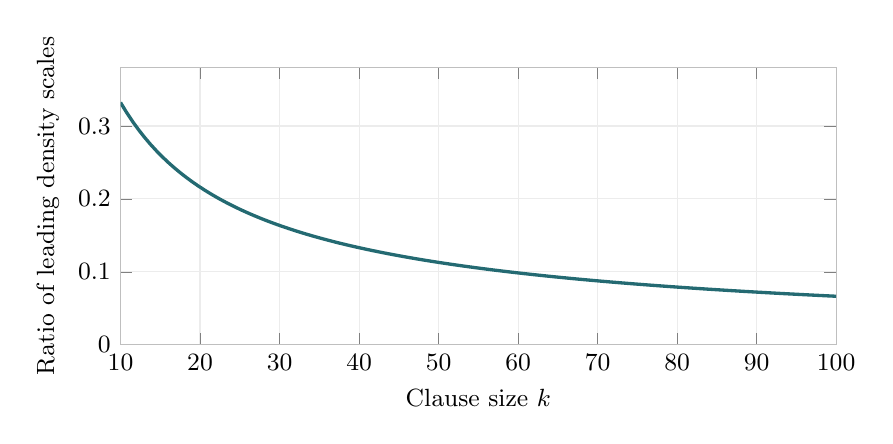
\begin{tikzpicture}
\begin{axis}[width=.88\linewidth,height=5.1cm,
 xmin=10,xmax=100,ymin=0,ymax=.38,
 xlabel={Clause size $k$},ylabel={Ratio of leading density scales},
 tick label style={font=\small},label style={font=\small},
 grid=major,grid style={gray!15},axis line style={gray!50},
 samples=120,domain=10:100]
\addplot[teal,very thick] {ln(x)/(x*ln(2))};
\end{axis}
\end{tikzpicture}
\caption{The analytic ratio $\log k/(k\log2)$. This compares the leading
large-$k$ expressions in \eqref{eq:fix} and \eqref{eq:largek}; it is not a
plot of measured algorithmic thresholds or a finite-$k$ guarantee.}
\label{fig:gap}
\end{figure}

Bresler and Huang prove obstructions for formally specified low-degree
polynomial and local algorithm classes at a constant multiple of this scale
\citep[Theorems 2.6 and 2.13]{bresler2021}. Their main low-degree theorem
uses $\alpha=\kappa2^k\log k/k$, $\kappa>\kappa_*\approx4.911$, and
sufficiently large $k$, with degree, normalization and success-probability
conditions. In particular, that theorem rules out a specified very high
success probability, not every nonzero success probability. The local-algorithm
result is stronger within its narrower class. Neither is a lower bound for
all polynomial-time algorithms, all CDCL implementations or finite-$k$ GPU
methods. The geometry of separated solution clusters and overlaps helps
explain these results; ``clustering implies hardness'' without a computational
model is only a heuristic.

\subsection{Proving UNSAT can be harder than predicting it}
At fixed density above the threshold, typical formulas are UNSAT. Efficiently
certifying this is a different question. A classical general polynomial-time
strong-refutation guarantee applies at
$m\ge\widetilde O(n^{k/2})$, with logarithmic factors and constants as in
\citet[Theorem 2.3 and Section 4]{allen2015}. For $3$-SAT this is about
$n^{3/2}$ clauses, much denser than the constant-density regime
$m\asymp4.27n$. It is a useful rigorous benchmark, not an efficient
near-threshold decision algorithm or a claim of optimality among all methods.

Resolution proof complexity supplies a concrete obstruction. Random $3$-CNF
formulas at suitable fixed UNSAT densities require exponential-size resolution
refutations whp; see \citet[Section 4.3]{ben2001}. This explains why
resolution-based search can struggle even when UNSAT is overwhelmingly
probable. The conclusion is specific to the proof system. Solvers with stronger
inference, extensions or inprocessing cannot all be identified with bare
resolution without checking the corresponding proof simulation.

\section{Practical algorithms and solver selection}
\label{sec:solvers}

\subsection{Complete solving: DPLL, CDCL and portfolios}
DPLL recursively chooses a variable, propagates forced values and backtracks
after a contradiction. Conflict-driven clause learning (CDCL) adds a derived
clause explaining a conflict, often jumps over irrelevant decisions, and
uses restarts, activity-based branching and clause-database management.
Preprocessing and inprocessing simplify the formula before and during search.
These engineering choices, rather than the best worst-case exponential base,
dominate many practical comparisons.

Kissat and CaDiCaL are strong, actively developed CPU baselines; their authors'
solver description documents the architecture and recent variants
\citep{biere2024}. CaDiCaL is also a natural starting point when an incremental
interface is required. For a one-off random-CNF experiment, compare an
optimized complete solver with a dedicated witness-search method. Use a
solver mode that records a compatible refutation when an independently
checkable UNSAT result is needed. Check witnesses against the \emph{original}
formula, including reconstruction after eliminated variables are restored.

The corrected SAT Competition 2026 results place
\texttt{satsuma-iter+kissat} first in the ordinary main overall ranking,
with 276 solved instances; the ordinary main SAT ranking has a different
winner, \texttt{satsuma-iter+ae-kissat-mab}, with 136
\citep[slides 13, 16 and 18]{satcomp2026}. These results support the
strength of the Kissat ecosystem, not a universal ranking on random $k$-SAT.
The competition mixes benchmark families and its 2026 tracks are not a
dedicated uniform-random-$k$-SAT comparison. Separate AI-category results
should not be silently merged into the ordinary ranking.

Parallel portfolios run diverse solver configurations and may exchange useful
clauses. A divide-and-conquer approach instead partitions the assignment
space. Both can reduce wall-clock time, but speedup depends on the instances
and includes additional CPU resources. Configuration should be tuned on a
training set and evaluated on unseen instances, rather than selected after
examining the test results \citep{hutter2017}.

\subsection{Witness search: local moves and probabilistic messages}
Stochastic local search keeps a complete assignment and repairs violated
clauses by flipping variables. Break counts measure how many satisfied
clauses a flip would destroy; noise and restarts help escape local traps.
\emph{probSAT} is a useful lightweight baseline with public source code
\citep{probsat}. More elaborate methods use clause weights and memory of
recent changes. For example, DCCASat combines two configuration-checking
rules to reduce cycling \citep{luo2014}. These methods can be effective on
large satisfiable random instances, but their failure to finish supplies no
UNSAT evidence.

Recent incomplete solvers increasingly combine logical propagation with local
repair. PALSAT, published at SAT 2026, progressively activates variables using
unit propagation and invokes local search to repair conflicts
\citep{jin2026}. Its comparisons with CCAnr variants and TaSSAT show gains
on recent competition and spectrum-repacking benchmarks. Those are structured
collections, so this result does not establish a new uniform-random-$k$-SAT
ranking. It does show why a present-day comparison should include newer hybrid
methods, rather than treating probSAT or the 2014 DCCASat results as a permanent
state of the art.

Belief propagation passes approximate local marginal information on the
variable--clause factor graph. Survey propagation (SP) instead aims to describe
the distribution of messages across solution clusters. Decimation fixes
strongly biased variables; backtracking survey propagation (BSP) can undo
some earlier choices. This is particularly relevant close to the random
satisfiability threshold, where correlations and frozen variables complicate
simple local search \citep{mmz2006,marino2016}.

BSP has impressive empirical results for random $3$-SAT, including formulas
with $10^6$ variables. Its empirical reach is much closer to the predicted
threshold than conservative rigorous small-$k$ guarantees. However, numerical
extrapolation of an algorithmic threshold is not a theorem that BSP succeeds
whp throughout the SAT phase. Nor is an SP fixed point itself a satisfying
assignment; any resulting Boolean assignment must still be checked.

\begin{table}[htbp]
\centering\small
\begin{tabularx}{\linewidth}{@{}L{.31\linewidth}Y@{}}
\toprule
Required output & Sensible first comparison \\
\midrule
SAT or UNSAT for each input & Complete CDCL baseline, with timeouts reported as unknown. \\
An assignment on likely-SAT random formulas & probSAT/local search versus BSP and CDCL. \\
A checkable UNSAT conclusion & Proof-logging complete solver plus a compatible checker. \\
Many independent random instances & CPU portfolio or batch parallelism; then a matched GPU comparison. \\
Native XOR/cardinality constraints & Solvers supporting those constraints directly; do not assume ordinary random-CNF results apply. \\
\bottomrule
\end{tabularx}
\caption{Recommendations for an initial experiment, not an assertion that
one implementation is best on every ensemble.}
\end{table}

\section{How large is practically feasible?}
\label{sec:scale}

A useful specification is $(k,n,\alpha,\text{ensemble},\text{task},
\text{time and hardware budget},\text{success target})$.
``A million variables'' alone says little. A sparse satisfiable formula
with a readily discoverable assignment and a near-critical UNSAT formula
can have radically different costs. General industrial SAT results also
cannot be read as uniform-random-$3$-SAT capacity estimates.

\subsection{Concrete evidence, including failures}
The historical Configurable SAT Solver Challenge used mixed random $3$-CNF
instances with 350 variables and 1493 clauses, and a satisfiable family with
1000 variables and 4260 clauses \citep[Appendix A.3]{hutter2017}. These
sizes indicate how small challenging complete-decision benchmarks can be;
they are not present-day hardware ceilings.

An especially informative comparison is the deliberately difficult
\texttt{Large\_Threshold} benchmark in \citet[Table 2]{luo2014}.
Table~\ref{tab:hardinstances} preserves the low success rates rather than
reporting only the largest instance size attempted.
\begin{table}[htbp]
\centering\small
\begin{tabular}{@{}rrrrr@{}}
\toprule
$k$ & $n$ & Density & probSAT solved & DCCASat solved \\
\midrule
3 & 15\,000 & 4.267 & 2/100 & 6/100 \\
4 & 2\,500 & 9.931 & 5/100 & 5/100 \\
5 & 600 & 21.117 & 2/100 & 9/100 \\
6 & 300 & 43.37 & 0/100 & 11/100 \\
7 & 150 & 87.79 & 28/100 & 43/100 \\
\bottomrule
\end{tabular}
\caption{Published 2014 local-search measurements: one run per instance,
5000-second cutoff, GNU/Linux on an Intel Core i7 at 2.4 GHz
(two cores reported in the setup). These are counts of witnesses found,
not proofs that the remaining formulas are UNSAT. The original benchmark
does not establish that every generated instance is satisfiable.}
\label{tab:hardinstances}
\end{table}

In contrast, \citet[Figures 3--5]{marino2016} report BSP solutions for
random $3$-SAT with $n=10^6$ at densities close to, but below, the predicted
transition, including analysis at $\alpha=4.262$. This is evidence that
million-variable \emph{search} can be feasible with a specialized method.
It is not a certificate of efficient complete decision at the transition.
The extrapolated value near $4.268$ in that paper is obtained by fitting
residual complexity; it must not be quoted as successful solving of
million-variable instances at that density. The cited figures also do not
provide a matched wall-clock and hardware comparison with Table~\ref{tab:hardinstances}.

The useful planning conclusion is therefore conditional: expect useful
near-critical complete-solver studies to begin at hundreds of variables;
thousands may already demand substantial budgets. For witness search below
the transition, thousands to hundreds of thousands are natural scales to
test, and a million is demonstrated in specialized published experiments.
These are starting expectations, not a machine-independent boundary or a
promise that every density in those ranges is tractable. Larger $k$ can be
hard at much smaller $n$, as the table illustrates.

\subsection{Input size and memory also constrain experiments}
There are $km=k\alpha n$ literal occurrences. Storing only one 32-bit signed
index per occurrence costs about $4k\alpha n$ bytes. At representative
densities this gives:
\begin{center}\small
\begin{tabular}{@{}rrrr@{}}
\toprule
$k$ & $n$ & $\alpha$ & Literal indices alone \\
\midrule
3 & $10^6$ & 4.267 & 51.2 MB \\
5 & $10^5$ & 21.117 & 42.2 MB \\
10 & $10^5$ & 708.936 & 2.84 GB \\
\bottomrule
\end{tabular}
\end{center}
These are arithmetic estimates in decimal units, not memory measurements.
Clause offsets, watches, occurrence lists, learned clauses, proof logs and
batched GPU states add overhead, sometimes substantial. Near the threshold,
$m$ grows exponentially with $k$; memory and input generation can become
limiting before the number of variables looks large.

\subsection{A reproducible first feasibility study}
The following is a \emph{proposed} pilot, not an experiment performed here.
For uniform random $3$-SAT, use densities $3.5,4.0,4.2,4.25,4.267,4.30,4.50$.
The values around $4.267$ are empirical landmarks, not a known exact
finite-$n$ threshold. For complete solving, begin with
$n=100,200,400,800$ and extend to $1600$ and beyond only after checking the
timeout rate. For witness search at the less critical densities, try
$n=10^3,10^4,10^5$ before committing to $10^6$.

Use at least 100 independently generated instances per cell if resources
permit, initially with a 60-second cutoff; repeat selected cells at 300 or
3600 seconds. These are budget choices, not asserted requirements for
success. Record generation seeds, solver versions, parameters, CPU cores,
RAM, GPU model and precision. Retain each raw result as SAT with a checked
witness, UNSAT with the stated checking status, or unknown. Report success
fractions and runtime distributions, including censored runs, rather than
only the median runtime among successes.

For $N$ sampled formulas, $S$ verified SAT and $U$ verified UNSAT outputs give
an empirical SAT-fraction interval
\begin{equation}
 [S/N,\;1-U/N].
 \label{eq:censor}
\end{equation}
This accounts for unknown answers in that sample; estimating the ensemble
probability additionally needs sampling uncertainty. Treating all timeouts
as UNSAT biases a threshold estimate downward. Successful-only datasets or
planted instances answer a different question.

\section{What GPUs can and cannot accelerate}
\label{sec:gpu}

GPUs are good at large batches of similar operations and less well suited to
irregular, sequential control flow. SAT offers both. Batched assignment
evaluation, independent local searches, message updates and some simplification
kernels expose parallel work. CDCL's trail, propagation dependencies, changing
clause database and divergent search paths make a straightforward wholesale
port difficult. The relevant question is therefore which computation is
accelerated and what fraction of total solving cost it represents.

\subsection{Published evidence}
\textbf{GPU inprocessing inside a complete solver.}
ParaFROST accelerates simplification and inprocessing and supports proof
logging \citep{osama2024}. Its experiments use an Intel Xeon Gold 6130,
96 GB RAM and a Titan RTX, with a 3600-second solving limit.
The CPU comparisons use a different Xeon E5-2630 machine, so the hardware
comparison is not fully matched.
The GPU version improves on its related CPU engine, but the paper also
reports that Kissat is faster overall on the evaluated collection.
This supports GPU acceleration of selected components, not an overall
advantage against every strong CPU solver. Proof production and checking
cost must be included when certification is the objective.

\textbf{Continuous local search.}
FastFourierSAT maps gradient computation for symmetric Boolean constraints
to GPU-friendly operations \citep{cen2025}. It is particularly relevant to
hybrid formulas containing native cardinality and XOR constraints.
The paper reports large kernel gains, but its ordinary CNF experiment is
cautionary: in a 1000-second test on satisfiable SAT Competition 2023
instances, its GPU variant solves 13 and its CPU variant 5. The corresponding
competition solvers solve those easy instances in roughly $0.04$--$1.07$
seconds. The GPU setup includes an RTX 3080 Ti. Thus a large acceleration
within one continuous-search method does not establish competitiveness with
CDCL on general CNF. The method is incomplete and cannot certify UNSAT.

\subsection{Recent preprints and comparison limits}
\textbf{TurboSAT.}
The November 2025 preprint combines GPU continuous search with CPU CDCL
\citep{dai2025}. On its 179-instance SAT Competition 2024 collection it
reports 165 solved within 5000 seconds, versus 143 for the chosen CaDiCaL
1.9.5 baseline. Experiments use a DGX GB200 system with up to two B200 GPUs
and 141 CPU threads. The method retains an unrestricted CDCL worker for
completeness. This is promising hybrid-system evidence, but it is not an
isolated GPU speedup: the CPU portfolio, hardware resources and configurations
also differ. These benchmarks are not a controlled random-$k$-SAT size study.

\textbf{Accelerated Fourier SAT.}
The June 2026 AFSAT preprint studies GPU implementation and throughput,
including hard random $3$-SAT and scaling across V100 GPUs
\citep{christopher2026}. It helps establish that this style of search can
benefit from parallel hardware. Throughput, however, must be combined with
the probability of finding a fully satisfying assignment to obtain a
time-to-solution comparison. Continuous objective values and almost-satisfying
outputs are insufficient; the benchmark must enforce zero violated clauses.

\begin{table}[htbp]
\centering\small
\begin{tabularx}{\linewidth}{@{}L{.27\linewidth}Y Y@{}}
\toprule
Approach & Evidence of benefit & Main limitation \\
\midrule
ParaFROST & GPU simplification within complete solving; published & Improvement over related CPU engine does not imply beating Kissat. \\
FastFourierSAT & Parallel gradients, especially hybrid constraints; published & Kernel gains and native-constraint advantages need not transfer to random CNF. \\
TurboSAT & More solves in a large hybrid system; preprint & Many CPU workers and GPUs confound a GPU-only comparison. \\
AFSAT & GPU throughput and random-$3$-SAT experiments; preprint & Throughput is not a complete-decision or UNSAT guarantee. \\
\bottomrule
\end{tabularx}
\caption{Four concrete GPU approaches. Publication status and benchmark
limitations are part of the comparison, not interchangeable speedup claims.}
\end{table}

\subsection{Recommendation for this project}
Establish a CPU baseline first. A GPU comparison is most informative for
large satisfiable random instances, many independent instances or restarts,
and batched message-passing or continuous-search experiments. Keep formula
generation, preprocessing, host--device transfer, compilation/warm-up,
assignment reconstruction and verification in the accounting. Compare
matched hardware budgets as well as raw wall-clock time; report CPU core
counts and GPU counts explicitly.

For near-threshold UNSAT certification, the checked literature provides no
basis for assuming that buying a GPU removes the principal difficulty.
GPUs may help specific kernels or portfolios, but a reduction in kernel
time cannot by itself overcome a search or proof-size bottleneck. A useful
reported speedup is the time to a verified answer on the same instances at
the same success target, not only flips per second or gradient evaluations
per second.

\Needspace{8\baselineskip}
\section{Comparison with the supplied geometry papers}
\label{sec:geometry}

\subsection{What the analogy explains}
The supplied paper \emph{Living on the edge} studies phase transitions for
randomly oriented convex cones and convex recovery problems \citep{almt2014}.
For a closed convex cone $C\subset\R^d$, its statistical dimension is
\[
 \delta(C)=\mathbb E\norm{\Pi_C(g)}^2,
 \qquad g\sim N(0,I_d),
\]
which extends linear dimension. If $C,K$ are closed convex cones and $Q$ is
a Haar-uniform orthogonal transformation, Theorem I gives, for
$0<\eta<1$ and $a_\eta=\sqrt{8\log(4/\eta)}$,
\begin{align*}
 \delta(C)+\delta(K)\le d-a_\eta\sqrt d
 &\ \Longrightarrow\ \mathbb P(C\cap QK\ne\{0\})\le\eta,\\
 \delta(C)+\delta(K)\ge d+a_\eta\sqrt d
 &\ \Longrightarrow\ \mathbb P(C\cap QK\ne\{0\})\ge1-\eta.
\end{align*}
This identifies both a transition location and a quantitative window through
an intrinsic geometric parameter. The theorem is not merely an empirical
fit to a transition curve.

The supplied \emph{Sharp Phase Transitions in Euclidean Integral Geometry}
develops concentration for weighted intrinsic-volume distributions of convex
bodies and applies it to integral-geometric questions
\citep[Theorems I--II and Section 4]{lotz2026}. Its central rotation and
rigid-motion volumes play the role of location parameters. This suggests
a productive conceptual comparison: identify a meaningful random variable,
prove concentration, and then link its typical value to feasibility.

Random $k$-SAT has a discrete version of a random covering problem. A clause
forbids precisely $2^{n-k}$ vertices of the Boolean cube; UNSAT means the
union of the forbidden subcubes covers every vertex. This perspective appears
directly in Carenini's proof. But its subcubes are sparse, coordinate-aligned
and strongly overlap. There is no Haar-random rotation, no given convex cone,
and no established statistical-dimension formula for $\alpha_k$ in this
comparison.

\subsection{Why the obvious convex relaxation loses the transition}
A clause with positive-variable set $P$ and negative-variable set $N$ can
be written exactly on Boolean points as
\[
 \sum_{i\in P}x_i+\sum_{j\in N}(1-x_j)\ge1.
\]
It is tempting to replace the Boolean cube by its convex hull and apply a
convex feasibility theorem. The following elementary observation shows why
that first step cannot work.

\begin{proposition}[The elementary clause relaxation cannot detect UNSAT]
\label{prop:lp}
Let $F$ be a CNF formula in which every clause contains at least two
literals. Replace each positive literal by $x_i$, each negative literal by
$1-x_i$, impose that each clause's literal sum is at least $1$, and relax
$x\in\{0,1\}^n$ to $x\in[0,1]^n$. This linear system is feasible for every
such $F$. In particular, feasibility of this relaxation is not equivalent
to satisfiability, even for proper $k$-CNF with fixed $k\ge2$.
\end{proposition}
\begin{proof}
Set every $x_i=1/2$. Every literal then has value $1/2$, so a clause with
$r\ge2$ literals has sum $r/2\ge1$. For an explicit UNSAT proper $k$-CNF,
take all $2^k$ sign patterns on the same $k$ variables. Every Boolean
assignment falsifies the clause with the opposite signs, so no assignment
satisfies the formula, although the same fractional point is feasible.
\end{proof}


The obstruction is specific to this relaxation. It does not rule out stronger
lifts, semidefinite or moment constraints, or a geometric description that
retains integrality. Such a program would first need a precise object, a
proved link between its geometric event and Boolean satisfiability, and the
correct distribution of orientations or constraints. Concentration of the
wrong feasible set would not resolve the random-$k$-SAT problem.

\noindent\textbf{Provenance.} Proposition~\ref{prop:lp} is an elementary
expository observation, recorded as P001 with state \texttt{proof-written};
it is not presented as novel or independently reviewed. The geometric
comparison supplies a direction for further study, not a proved transfer
of either supplied geometric theorem.

\section{Research priorities and source scope}
\label{sec:outlook}

For an initial random-$k$-SAT project, three next steps are concrete.
First, review the supplied threshold proof in detail, checking its stopping-time
and model-transfer arguments and the dependencies of the convergence criterion.
The newer window and $4.268$ upper-bound manuscripts should be assessed
separately, including any claimed formal artifacts. Second, run the modest
CPU feasibility pilot in Section~\ref{sec:scale}, keeping search and complete
decision results separate. Third, if the geometric analogy is pursued,
specify a relaxation or discrete invariant that survives the obstruction in
Proposition~\ref{prop:lp} before attempting a concentration theorem.

The algorithmic frontier is best expressed as a collection of questions.
How far into the satisfiable phase can one guarantee polynomial-time witness
search? Which computational models explain the observed barrier? Can random
UNSAT formulas at constant density be efficiently certified by stronger
methods? For small fixed $k$, how precisely can the threshold location and
finite-size bias be determined? The reviewed sources address parts of these
questions; the recent preprints do not supply a complete practical solution.

\subsection{The supplied inventory and added literature}
The repository originally supplied four PDFs. \texttt{TR26-229.pdf} is
Carenini's October 2026 random-$k$-SAT preprint. \texttt{iau005.pdf} is
Amelunxen--Lotz--McCoy--Tropp, and \texttt{sharp-phase.pdf} is Lotz--Tropp.
The file \texttt{montanari-phase.pdf} is actually Montanari and Wang's
\emph{Phase Transitions for Feature Learning in Neural Networks}
\citep{montanari2026}; it is not a second random-$k$-SAT background paper.
It has therefore not been used as evidence for a SAT theorem. The background
coverage here is supplied by the additional primary sources in the bibliography.

Literature and software results were checked through 10 October 2026.
The exposition revision of 11 October adds the elementary clause-count
proof and its teaching-note reference, and expands the clause-process definition.
The coverage is targeted, not a claim of an exhaustive literature search.
The source registry records stable S identifiers, versions, local originals,
precise theorem/table locations and the scope of each reading. Checking a
stated theorem and its hypotheses is distinguished from checking its proof;
reported computational and Lean artifacts were not rerun.

The article, bibliography and P001--P002 fragments are editable LaTeX. The repository
command \texttt{make report} produces the PDF. The project status and source
manifest identify the dated version; earlier template material is archived.
No new solver measurements are included. Consequently the immediate missing
evidence for a hardware-specific size recommendation is the local pilot,
not another extrapolation from an unrelated benchmark.


\ifreportbibliography
  \clearpage
  \phantomsection
  \addcontentsline{toc}{section}{References}
  \begingroup
    \small\raggedright
    \bibliographystyle{plainnat}
    \bibliography{references}
  \endgroup
\else
  \section*{References}
  \phantomsection
  \addcontentsline{toc}{section}{References}
  No sources are cited in this template. Add verified entries to
  \texttt{references.bib} and enable the bibliography in
  \texttt{metadata.tex} when initializing the project.
\fi
\end{document}
